\chapter{Extrinsic semiconductors}
In order to increase the electron density $n$ (in CB) or hole density $p$ (in VB), one needs to dope a semiconductor. Meaning impurities get introcued in the semiconductor.

\section{Doping}
If we look at Silicon, a group IV element, we know it has 4 electrons in bonding. \par If we now would substitute Si by a group III element (B, Ga, In), which is introducing impurities, we see that there is an electron less in the crystal. This means we introduced a holes in the crystal, and this will be called a p-type doping. \par If we now would substitute Si by a group V element (P, As, Sb), which is introducing impurities, we see that there is an extra electron in the crystal. This means we introduced an electron in the crystal, and this will be called a n-type doping. \\ \par
If we now look at the energy diagrams we notice the following:
\begin{figure}
	\centering
	\begin{tikzpicture}
		\draw[black]	(1, 3.5) node[]{Intrinsic};
		\draw[-, black, very thick]	(0, 3) to (2, 3) node[right]{$E_c$};
		\draw[-, gray, very thick]	(0, 2) to (2, 2) node[right]{$\mu$};
		\draw[-, black, very thick]	(0, 1) to (2, 1) node[right]{$E_v$};

		\draw[black]	(4, 3.5) node[]{Donor};
		\draw[-, black, very thick]	(3, 3) to (5, 3) node[right]{$E_c$};
		\draw[--, gray, very thick]	(3, 2.7) to (5, 2.7) node[right]{$E_D$};
		\draw[-, black, very thick]	(3, 1) to (5, 1) node[right]{$E_v$};

		\foreach \x in {1,...,7} {
			\filldraw[blue]	(3 + \x/4, 2.7) circle (2pt);
		}

		\draw[black]	(7, 3.5) node[]{Acceptor};
		\draw[-, black, very thick]	(6, 3) to (8, 3) node[right]{$E_c$};
		\draw[--, gray, very thick]	(6, 1.3) to (8, 1.3) node[right]{$E_A$};
		\draw[-, black, very thick]	(6, 1) to (8, 1) node[right]{$E_v$};

		\foreach \x in {1,...,7} {
			\draw[blue]	(6 + \x/4, 1.3) circle (2pt);
			\filldraw[blue]	(6 + \x/4, 0.7) circle (2pt);
		}
	\end{tikzpicture}
	\caption{Intrinsic, donor and acceptor Si energy diagrams}
	\label{fig:donor_acceptor}
\end{figure}
We notice donor and acceptor levels. At $0K$, these states are completely filled with electrons or holes, respectively. Now, at finite temperatures, these electrons or holes jump to the CB or VB (respectively). As we know, an electron that goes away, leaves a hole. Thus when jumping from the $E_D$ to $E_C$, a hole is left in the donor level. When a, electron jumps from the VB to the $E_A$ band, it fills a hole in $E_A$ and leaves a hole behind. Notice the donor/acceptor energy level of the dopant.\\ \par
The question can now arise: what are these donor and acceptor energies? \\
We know that near the impurity in the silicon lattice, the electron/hole will see a coulomb potential
\begin{equation}
	V_{dopant} = \pm \frac{e^2}{4\pi\epsilon_{Si}r}
\end{equation}
which is a hydrogen spectrum. Thus the acceptor and donor energy level is more like a spectrum where the $E_{ionization}$ of the hydrogen model ($\apprx 13.6 eV$) is the difference between $E_D$ and $E_c$ or $E_A$ and $E_v$. These dopants act like mini-hydrogen atoms. We will come back to this later on.

\subsection{Donor and acceptor energy levels}
\subsubsection{Occupation probability of acceptor/donor energy levels}
It turns out that the occupation probabilty for these levels is also given by a Fermi-Dirac distribution:
\begin{align}
	f_D(E_D) &= \frac{1}{1+\frac{1}{g_d}e^{\frac{E_D-\mu}{k_BT}}} \\
	f_A(E_A) &= \frac{1}{1+g_ae^{\frac{E_A-\mu}{k_BT}}} \\
\end{align}
Notice the $g_i$ factor is a degeneration factor for the energy bands, these can be found in tables.\\
Now we can calculate the chemical potential, because with these donor/acceptor states, the position of the chemical potential will change.

\subsubsection{Determining the chemical potential for doped semiconductor}
For the intrinsic case, remember we used the fact that $n = p$ to calculate the chemical potential. For the extrinsic case, we will use following rule to obtain charge neutrality
\begin{align}
	N_D^* + p &= N_A^- + n \\
	\text{Where}\qquad N_C^+ &= \left[1 - f_D(E_D)\right]N_D \nonumber \\
	N_A^- &= f_A(E_A)N_A \nonumber
\end{align}
Which, after substitution, leads to:
\begin{equation}
	\frac{N_D}{1+g_de^{\frac{\mu - E_D}{k_BT}}} + N_VF_{1/2}\left(\frac{\mu - E_v}{K_BT}\right) = \frac{N_A}{1+g_ae^{\frac{E_A-\mu}{k_BT}}} + N_CF_{1/2}\left(\frac{E_c - \mu}{K_BT}\right)
\end{equation}
This way we can determine $\mu(T)$. As we see, there is a temperature dependence of $N_D^+$, $n$ and $\mu$. We look at this in the next part.\\ \par
\textbf{Temperature dependence of $\frac{n}{N_D}$}\\
We will look at temperatures between $0K$ and $500K$ and we suppose there is $N_A = 0$ and $N_D \neq 0 >> n_i$. As we see in figure \ref{fig:tempdependence}: in the freeze out region, we get an increase of electrons in the conduction band that come from the donor energy levels (the dopants). After a while if all donor electrons are excited, the electrons from the substrate will excite, too. \\ \par
If we take $T \rightarrow 0$, then we can say
\begin{equation}
	\mu = \frac{E_D + E_c}{2} + \frac{k_BT}{2}\ln\frac{N_D}{g_dN_c}
\end{equation}
\nt{For a acceptor semiconductor ($N_D = 0$, $N_A \neq 0 >> n_i$), we will get following equation for $\mu$:
\begin{equation}
	\mu = \frac{E_A + E_v}{2} + \frac{k_BT}{2}\ln\frac{N_A}{g_aN_v}
\end{equation}
}
Further information is given in the course book. Part of the exercise session covers deriving the chemical potential at different temperatures.
\begin{figure}
	\centering
	\begin{tikzpicture}
		\draw[->, black]	(0, 0) to (0, 3) node[left]{$\frac{n}{N_D}$};
		\draw[->, black]	(0, 0) to (10, 0) node[right]{$T$};

		\draw[black]	(1, 3.5) node[]{Freeze out};
		\draw[-, black, very thick]	(0, -1) 	node[left]{$E_c$} to (2, -1);
		\draw[--, gray, very thick]	(0, -1.3)	node[left]{$E_D$} to (2, -1.3);
		\draw[-, black, very thick]	(0, -3) 	node[left]{$E_v$} to (2, -3);

		\foreach \x in {1,...,7} {
			\filldraw[blue]	(\x/4, -1.3) circle (2pt);
			\filldraw[blue]	(\x/4, -3) circle (2pt);
		}


		\draw[black]	(4, 3.5) node[]{Saturation region};
		\draw[-, black, very thick]	(3, -1) to (5, -1);
		\draw[--, gray, very thick]	(3, -1.3) to (5, -1.3);
		\draw[-, black, very thick]	(3, -3) to (5, -3);

		\filldraw[blue]	(3 + 5/4, -0.7) circle (2pt);
		\draw[blue] (3 + 5/4, -1.3) circle (2pt);
		\foreach \x in {1,...,4} {
			\filldraw[blue]	(3 + \x/4, -1.3) circle (2pt);
		}
		\foreach \x in {6,...,7} {
			\filldraw[blue]	(3 + \x/4, -1.3) circle (2pt);
		}
		\foreach \x in {1,...,7} {
			\filldraw[blue]	(3 + \x/4, -3) circle (2pt);
		}

		\draw[black]	(7, 3.5) node[]{Intrinsic region};
		\draw[-, black, very thick]	(6, -1) to (8, -1);
		\draw[--, gray, very thick]	(6, -1.3) to (8, -1.3);
		\draw[-, black, very thick]	(6, -3) to (8, -3);

		\foreach \x in {1,...,7} {
			\draw[blue]	(6 + \x/4, -1.3) circle (2pt);
			\filldraw[blue]	(6 + \x/4, -3) circle (2pt);
			\filldraw[blue]	(6 + \x/4, -0.7) circle (2pt);
		}

		\draw[-, black, very thick]	(9, -1) to (11, -1);
		\draw[--, gray, very thick]	(9, -1.3) to (11, -1.3);
		\draw[-, black, very thick]	(9, -3) to (11, -3);

		\foreach \x in {1,...,7} {
			\draw[blue]	(9 + \x/4, -1.3) circle (2pt);
			\draw[blue]	(9 + \x/4, -3) circle (2pt);

			\filldraw[blue]	(9 + \x/4, -0.7) circle (2pt);
			\filldraw[blue]	(9 + \x/4, -0.4) circle (2pt);
		}

		\draw[dashed, red, thick]	(2.5, 3) to (2.5, -3)
										(5.5, 3) to (5.5, -3)
										(8.5, 3) to (8.5, -3);

		\draw[black]	(0, 0)	node[below]{$0$};
		\draw[red]	(2.2, 0)	node[below]{$100$};
		\draw[red]	(5.2, 0)	node[below]{$300$};
		\draw[red]	(8.2, 0)	node[below]{$500$};

		\draw[red, very thick]	plot[samples=200, domain=0:2.5] (\x, \x*\x/4);
		\draw[red, very thick]	plot[samples=200, domain=2.5:5.5] (\x, 2.5*2.5/4);
		\draw[red, very thick]	plot[samples=200, domain=0:5.1] (\x+5.5, \x*\x/14 + 2.5*2.5/4);

		\draw[dotted, red, fine]	(0, 2.5*2.5/4) node[left]{$1$} to (2.5, 2.5*2.5/4);
	\end{tikzpicture}
	\caption{The temperature dependence of $\frac{n}{N_D}$}
	\label{fig:tempdependence}
\end{figure}

\chapter{Dynamics of charge carriers}
\section{The velocity of an electron}
To know what the velocity is, we need to look at quantum mechanics. If we have a Block hamiltonian (with periodic $V(\vec{r})$), we can define the velocity operator.
\begin{equation}
	\hat{\vec{v}} = \frac{d\hat{\vec{r}}}{dk} = \frac{1}{i\hbar}\left[\hat{\vec{r}}, \hat{H}\right] = -\frac{i\hbar}{m}\vec{\nabla} = \frac{\hat{\vec{p}}}{m}
\end{equation}
Wat can I say about this velocity operator? Specifically, the expectation value of this velocity:
\begin{align}
	<\hat{\vec{v}}> &= <\psi|\hat{\vec{v}}|\psi> = -\frac{i\hbar}{m}\int_{}^{} d^3x\, \psi^*(\vec{r}) \vec{\nabla} \psi(\vec{r})
\end{align}
Because we have a periodic crystal, we can define $\psi$ as
\begin{equation}
	\psi_{\vec{k}}(\vec{r}) = u_{\vec{k}}(\vec{r})e^{i\vec{k}\cdot\vec{r}}
\end{equation}
Then, by using $\int_{}^{}d^3x\, \abs{u_{\vec{k}}(\vec{r})}^2 = 1$ we can define the expectation value as
\begin{equation}
	<\hat{\vec{v}}> = \frac{\hbar\vec{k}}{m} - \frac{i\hbar}{m}\int_{}^{}d^3x\, u_{\vec{k}}^*(\vec{r}) \vec{\nabla} u_{\vec{k}}(\vec{r}) \label{eqn:velocity_guess}
\end{equation}
By making use of the Schrödinger equation
\begin{equation*}
	\left\{\frac{\hbar^2}{2m}\left(-\vec{\nabla} + \vec{k}\right)^2 + V(\vec{r})\right\}u_{\vec{k}}(\vec{r}) = E(\vec{k})u_{\vec{k}}(\vec{r})
\end{equation*}
it us possible to show that
\begin{equation*}
	\frac{i\hbar}{m}\int_{}^{}d^3x\, u_{\vec{k}}^*(\vec{r}) \vec{\nabla} u_{\vec{k}}(\vec{r}) = \frac{\hbar\vec{k}}{m} - \frac{1}{\hbar}\vec{\nabla}_{\vec{k}}E(\vec{k})
\end{equation*}
In order that equation \ref{eqn:velocity_guess} becomes
\begin{equation}
	<\hat{\vec{v}}> = \frac{1}{\hbar}\vec{\nabla}_{\vec{k}}E_n(\vec{k})
\end{equation}
which is the equation for group velocity, this is the velocity of a wave packet. Say you have an energy dispersion relation and you construct a wave packet representing electrons with different k values, then the maximum this wavepacket is moving is given by the group velocity.
\thm{Group velocity}{
	Take a 1D bloch wave function: $\psi_k(x) = u_k(x)e^{ikx}$.
	Then we can construct a wave packet in the first BZ ($-\pi/a\dots \pi/a$):
	\begin{equation*}
		\psi(x, t) = \int_{-\pi/a}^{\pi/a}dk\, A(k)\psi_k(x)e^{-\frac{i}{\hbar} E(k)t}
	\end{equation*}
	If we fill in the expression for $\psi$ and use a taylor expansion for the exponential function one gets:
	\begin{align*}
		\psi(x, t) &\approx \int_{-\pi/a}^{\pi/a}dk A(k)u_k_0(x)e^{i\left(k_0x - \frac{E(k_0)t}{\hbar}\right)}e^{i(k-k_0)\left(x - \left\frac{dE}{dk}\right|_k_0\frac{t}{\hbar}\right)} \\
		&= e^{i\left(k_0x - \frac{E(k_0)t}{\hbar}\right)}u_k_0(x) \int_{-\pi/a}^{\pi/a}dk A(k)e^{i(k-k_0)\left(x - \left\frac{dE}{dk}\right|_k_0\frac{t}{\hbar}\right)}
	\end{align*}
	The we can describe the probability density function as:
	\begin{equation*}
		\abs{\psi(x, t)}^2 = P(x, t) = \dots
	\end{equation*}
	Because we have a very sharp peak around $k_0$ in the function $A(k)$, this integral will have a stationary phase condition. Meaning we will reach a maximum of our integral if
	\begin{equation*}
		x - \left\frac{dE}{dk}\right|_{k=k_0}\frac{t}{\hbar} = 0 \quad \Righarrow \quad x = \left\frac{dE}{dk}\right|_{k=k_0}\frac{t}{\hbar}
	\end{equation*}
	We can represent this in the vollowing way:
	\begin{center}
		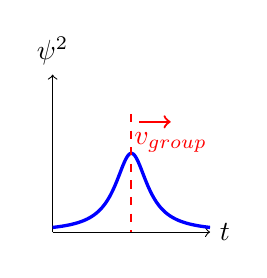
\begin{tikzpicture}
			\draw[->, black]	(0, 0) to (2, 0) node[right]{$t$};
			\draw[->, black]	(0, 0) to (0, 2) node[above]{$\abs{\psi}^2$};

			\draw[blue, very thick]	plot[samples=200, domain=-4:4] ({\x/4 + 1}, {1/(1 + \x*\x)});

			\draw[red, dashed, thick] 	(1, 1.5) to (1, 0);
			\draw[red, thick, ->]		(1.1, 1.4) to (1.5, 1.4) node[below]{$v_{group}$};
		\end{tikzpicture}
	\end{center}
	This wave moves, with a velocity, the group velocity
	\begin{equation*}
		v = \frac{dx}{dt} = \left\frac{dE}{dk}\right|_{k=k_0}\frac{1}{\hbar}
	\end{equation*}
}
Now what is interesting is that this group velocity comes form a wave packet, but we didn't construct a wave packet! When calculating the expectation value of the velocity of the electrons, these electrons in these eigenstates move with a group velocity. This is not a trivial result. The only difference between the two is that the group velocity for a wave packet is only valid nearby this $A(k)$ peak (at $k_0$), whereas the group velocity here is valid for any $\vec{k}$.

\subsection{The acceleration of an electron}
This is given by
\begin{equation}
	\frac{d}{dt}<\vec{v}> \,= \,\frac{d}{dt}\left(\frac{1}{\hbar}\vec{\nabla}_{\vec{k}}E(\vec{k})\right) = 0 = \vec{a} =\, <\vec{a}>
\end{equation}

\section{The velocity of an electron - with external field} \label{sec:eff_mass_th}
In this case, the hamiltonian becomes
\begin{equation}
	\hat{H} = \frac{\hat{p}^2}{2m} + V_C(\vec{r}) + V_{ext}(\vec{r}, t) \label{eqn:hamiltonian_seq_velocity}
\end{equation}
If we want to inlcude these external fields, we need to solve the time dependant Schrödinger equation. This isn't trivial, but there is a trick. By using a "effective" Schrödinger equation defined by the following theorem we can solve this problem easier.
\thm{Effective mass theorem}{
	It can be shown that
	\begin{equation}
		\left[\hat{E}_n(-i\vec{\nabla}) + V_{ext}(\vec{r}, t)\right]\psi(\vec{r}, t) = i\hbar\frac{\delta\psi(\vec{r}, t)}{\delta t} \label{eqn:electron_velocity}
	\end{equation}
	We obtain this formula by replacing $\vec{k} \rightarrow -i\vec{\nabla}$ in $E_n(\vec{k})$.
}
\begin{myproof}
	\begin{equation}
		\psi(\vec{r}, t) = \sum_{\vec{k}}^{}c_n(\vec{k}, t)\psi_{\vec{k}}(\vec{r}) \qquad \text{with } \psi_{\vec{k}}(\vec{r}) = u_{\vec{k}}e^{i\vec{k}\cdot\vec{r}}
	\end{equation}
	Maybe you can see that equation \ref{eqn:electron_velocity} is typically valid for one specific band (see subscript $n$). this also means that when Ido the expansion, we don't want to refer to all the bands. Therefore we make an approximation where we assume that the solution is restricted to a single band. Next, the only electrons we are interested in are the ones in the vicinity of the minimum of the conduction band (or the maxima of the valence band for holes).
	Then the approximations we make are:
	\begin{enumerate}
		\setlength\itemsep{0pt}
		\item Only one band at at time
		\item Only $\vec{k}$-values near band extrema
	\end{enumerate}
	Thus our wave function will become
	\begin{align}
		\psi(\vec{r}, t) &= \sum_{\vec{k}}^{}c_{\vec{k}}(t)\psi_{\vec{k}}(\vec{r}) \label{eqn:above} \\
		\ref{eqn:hamiltonian_seq_velocity} \text{ in } \ref{eqn:above} \qquad \Rightarrow \quad & \sum_{\vec{k}}^{} c_{\vec{k}}(t)\left[-\frac{\hbar^2}{2m}\nabla^2 + V_C + V_{ext}\right]\psi_{\vec{k}}(\vec{r}) = i\hbar\frac{\delta \psi}{\delta t}
	\end{align}
	If we look at the total hamiltonian acting on the eigenfunction of the Bloch hamiltonian meaning the wavevector is an eigenfunction of the total hamiltonian. Thereby we can replace the hamiltonian by the eigenenergy.
	\begin{equation}
		\rightarrow \quad \sum_{\vec{k}}^{} c_{\vec{k}}(t)\left[E(\vec{k}) + V_{ext}\right]\psi_{\vec{k}}(\vec{r}) = i\hbar\frac{\delta \psi}{\delta t} \label{eqn:toconcludeproof}
	\end{equation}
	Because $E(\vec{k})$ is periodic, we can make a fourier expansion in k-sapce:
	\begin{align}
		E(\vec{k}) &= \sum_m^{}E_me^{i\vec{R}_m\cdot\vec{k}} \qquad \text{with $\vec{R}_m$ a lattice vector}\\
		& \text{substitute } \vec{k} \rightarrow i\vec{\nabla} \nonumber \\
		\Rightarrow \quad \hat{E}(-i\vec{\nabla}) &= \sum_m^{}E_me^{i\vec{R}_m\cdot\vec{\nabla}} \label{eqn:engery_nabla}
	\end{align}
	When letting the exponential act on a function we get (this can be proved by a taylor expansion of the exponential):
	\begin{equation}
		e^{i\vec{R}_m\cdot\vec{\nabla}}\psi_{\vec{k}}(\vec{r}) = \psi_{\vec{k}}(\vec{r} + \vec{R}_m)
	\end{equation}
	If we now let equation \ref{eqn:engery_nabla} act on the Bloch wave function we get the following:
	\begin{align}
		\hat{E}(-i\vec{\nabla})\psi_{\vec{k}}(\vec{r}) &= \sum_m^{}E_me^{i\vec{R}_m\cdot\vec{\nabla}}\psi_{\vec{k}}(\vec{r}) \\
		&= \sum_m^{}E_m\psi_{\vec{k}}(\vec{r} + \vec{R}_m) \\
		\text{Using the Bloch wavefunction property }	\qquad &= \sum_m^{}E_me^{i\vec{R}_m\cdot\vec{k}}\psi_{\vec{k}}(\vec{r}) \\
		&= E(\vec{k})\psi_{\vec{k}}(\vec{r})
	\end{align}
	What we now have showed is that the operator $\hat{E}(-i\vec{\nabla})$ acting on the eigenstates of the Hamiltonian gives as eigenvalues, the eigenenrgies of the Hamiltonian. Now we can safely write that $E(\vec{k}) = \hat{E}(-i\vec{\nabla})$. \\
	We can now rewrite equation \ref{eqn:toconcludeproof} as
	\begin{align}
		\sum_{\vec{k}}^{} c_{\vec{k}}(t)\left[E(-i\vec{\nabla}) + V_{ext}\right]\psi_{\vec{k}}(\vec{r}) &= i\hbar\frac{\delta \psi}{\delta t} \\
		\left[E(-i\vec{\nabla}) + V_{ext}\right]\sum_{\vec{k}}^{} c_{\vec{k}}(t)\psi_{\vec{k}}(\vec{r}) &= i\hbar\frac{\delta \psi}{\delta t} \\
		\left[E(-i\vec{\nabla}) + V_{ext}\right]\psi(\vec{r}, t) &= i\hbar\frac{\delta \psi(\vec{r}, t)}{\delta t}
	\end{align}
\end{myproof}
\nt{This is only valid if we stick in the conduction or valence band.}
